%% Empirical Software Engineering (Springer) submission
%% Class + styles from the Springer Nature LaTeX template v3.1.
%% Compile: pdflatex -> bibtex -> pdflatex -> pdflatex
\documentclass[sn-basic,Numbered]{sn-jnl}

\usepackage{graphicx}
\usepackage{multirow}
\usepackage{amsmath,amssymb,amsfonts}
\usepackage{amsthm}
\usepackage{booktabs}
\usepackage{xcolor}
\usepackage{textcomp}
\usepackage{url}

\theoremstyle{definition}
\newtheorem{definitionx}{Definition}
\theoremstyle{plain}
\newtheorem{proposition}{Proposition}

\raggedbottom

\begin{document}

\title[An Evidence-Bound Runtime Contract for LLM Narration]{%
Prompts Are Advisory, Schemas Are Enforcement:\\
An Evidence-Bound Runtime Contract for Claim-Faithful\\
LLM Narration of Machine-Learning Pipeline Evidence}

\author*[1]{\fnm{Hakan} \sur{Sabuni\c{s}}}\email{hakan.sabunis@std.medipol.edu.tr}
\author[1]{\fnm{Yusuf} \sur{\"Unl\"u}}\email{yusuf.unlu@std.medipol.edu.tr}
\author[1]{\fnm{Selim} \sur{Aky\"ok\"u\c{s}}}\email{sakyokus@medipol.edu.tr}

\affil[1]{\orgdiv{School of Engineering and Natural Sciences},
\orgname{Istanbul Medipol University},
\orgaddress{\city{Istanbul}, \country{T\"urkiye}}}

%%%%%%%%%%%%%%%%%%%%%%%%%%%%%%%%%%%%%%%%%%%%%%%%%%%%%%%%%%%%%%%%%%%%%%%
\abstract{%
\textbf{Context.} Software tools increasingly place a large language model
(LLM) between a deterministic analysis and the engineer who acts on it. The
model reads structured evidence a tool measured and explains it in prose. When
the explanation invents a column, a defect, or a number, the engineer acts on
something that was never observed.

\textbf{Objective.} We ask whether this particular failure can be
\emph{prevented} rather than statistically reduced, and whether the prevention
buys anything a general-purpose guardrail toolkit does not already provide.

\textbf{Method.} We identify a class of narration tasks we call
\emph{evidence-closed}: the set of citable entities and checkable quantities is
finite and machine-enumerable at the moment of the narration call, which makes
faithfulness decidable. We build a two-tier \emph{evidence-bound runtime
contract} on that property and ship it in the production narrator of
\textbf{mlcompass}, an open-source ML-pipeline assistant. We evaluate it with a
controlled experiment ($N=200$ per cell, seven arms, 1{,}400 live responses),
a six-variant paraphrase sweep ($N=100$ per variant, 600 responses), and a
pre-registered $4\times3\times4$ A/B benchmark of downstream code quality
(144 runs, four models, three datasets).

\textbf{Results.} Three findings. (i)~The failure is not the one the
literature names: decomposing every flagged response shows the bare narrator
\emph{misfiles} real evidence names at 4--71\,\% while \emph{inventing} names
at 0--7\,\%, and the two rates move independently across wordings. (ii)~The
outer loop is not the contribution: Guardrails~AI with stock validators leaves
35.0\,\% (70/200); the same toolkit, the same reask budget, running our
deterministic validators leaves 0/200. (iii)~Downstream, flagged defects fall
33~$\rightarrow$~8 across four models, and a fourth arm isolates the cause --- a
second attempt \emph{without} the tool's findings fixes nothing (33~$\rightarrow$~35,
zero defects repaired in 35 runs).

\textbf{Conclusions.} For evidence-closed narration, faithfulness on the
validated channels is enforceable by construction and independent of the
provider. What a rate-reduction defence cannot give, and what we measure, is a
worst-case guarantee that survives rewording. We report three defects we found
in our own instruments, the corrections they forced, and the two published
figures that this replication does not reproduce.
}

\keywords{Large language models, Hallucination, Faithfulness, Tool use,
Constrained generation, Data leakage, Empirical evaluation}

\maketitle
%%%%%%%%%%%%%%%%%%%%%%%%%%%%%%%%%%%%%%%%%%%%%%%%%%%%%%%%%%%%%%%%%%%%%%%

\section{Introduction}\label{sec:intro}

Machine-learning practice runs on single-purpose tools. A profiling library
inspects the dataset~\cite{ydata}, experiment trackers record training
runs~\cite{mlflow,tensorflow}, automated model search picks an
estimator~\cite{autosklearn}. Each covers one slice of the pipeline and none
tells the engineer what the results \emph{mean}. The now-standard answer is
agentic: put an LLM on top, let it call the tools, read their structured
output, and explain --- the pattern formalised by ReAct~\cite{react} and
Toolformer~\cite{toolformer} and operationalised by tool-integration
standards~\cite{mcp}.

The trouble is that LLMs hallucinate~\cite{ji,huang}, and assistants built on
the same foundation models~\cite{codex} still fail real software tasks at
substantial rates~\cite{swebench}. In an advisory ML setting the failure takes
a specific shape. The narrated object is \emph{structured evidence} --- a
dictionary of facts a deterministic tool actually measured --- and the narrator
can report members of it that are not there: a column the data does not
contain, a defect nobody detected, a number that contradicts the report. The
cost is concrete, because a wrong diagnosis delivered fluently is worse than no
diagnosis: the practitioner acts on it.

This paper is built on one observation about that setting. What the narrator
may cite is \emph{finite and machine-enumerable at the moment of the call}. We
name the class:

\begin{definitionx}[Evidence-closed narration]\label{def:closed}
A narration task is \emph{evidence-closed} if the set of citable entities and
verifiable quantities is finite and machine-enumerable at the moment of the
narration call.
\end{definitionx}

Once a task is evidence-closed, faithfulness checking stops being a modelling
problem. Entity citations become set-membership tests, quantitative claims
become numeric comparisons, and coverage of the critical finding is one more
membership test. The check is \emph{decidable}, which changes the sensible goal
from \emph{mitigation} --- pushing a probability down --- to \emph{prevention}:
making an unfaithful answer impossible to return on the channels that carry the
actionable content.

Constrained generation looks like the natural instrument. Outlines~\cite{outlines},
LMQL~\cite{lmql}, grammar-constrained decoding~\cite{gcd} and
Guidance~\cite{guidance} restrict what a model may emit during decoding, and
provider tool-use APIs validate calls against a declared JSON
schema~\cite{structured}. Two things go wrong here. Decoding-time enforcement
needs the token distribution, and commercial APIs do not expose it. A per-call
schema, in turn, only helps if the provider's enforcement is trusted, and for a
safety claim it should not be.

\paragraph{The artifact.} Our answer is a two-tier \textbf{evidence-bound
runtime contract}. \emph{Tier~A} generates the \texttt{enum} domains of the
narrator's tool-input fields from the deterministic evidence dictionary at call
time, constraining generation as far as a closed API allows. \emph{Tier~B}
takes over where trust ends: plain code re-checks the returned answer on three
channels --- entity soundness, value soundness of structured
\{column, statistic, value\} claims, and completeness with respect to the
top-ranked candidate --- with corrective retry, residual stripping, and
omission flagging. It is not a prototype. It runs in the production narrator of
\textbf{mlcompass}, an open-source (MIT) ML-pipeline assistant, guarding the
investigation that fires when an evaluation metric looks too good to be true
($R^2>0.999$, $\mathrm{AUC}>0.995$), the classic signature of data
leakage~\cite{leakage}.

\paragraph{On reporting our own mistakes.} Three of the results below
contradict what we believed at the point the study began. The failure mode is
not the one we set out to measure (Section~\ref{sec:rq1}); the downstream
effect could not initially be attributed to the tool, and a fourth arm was
needed to attribute it (Section~\ref{sec:rq5}); and three defects in our own
measuring instruments produced numbers we had already reasoned from
(Section~\ref{sec:instruments}). We report each in the body rather than an
appendix, with the superseded measurements preserved in the replication package
beside their corrections, because an instrument defect found and reported by
the authors is evidence about the instrument, and one found by a reader is
evidence about the authors.

\paragraph{Research questions.}
\begin{description}
\item[RQ1] How does an unconstrained narrator of evidence-closed material
actually fail, and does the failure match the name the literature gives it?
\item[RQ2] Does the contract prevent that failure on the validated channels?
\item[RQ3] Does it do so better than the state-of-the-art alternatives a
practitioner would otherwise reach for?
\item[RQ4] Can a prompt-level defence be certified from observed compliance?
\item[RQ5] Does the tool change what an LLM downstream actually produces, and
if so, which part of it does the work?
\end{description}

\paragraph{Contributions.}
\begin{enumerate}
\item \textbf{The evidence-closed class} (Definition~\ref{def:closed}) with the
two facts the design rests on: faithfulness verification is linear-time
(Proposition~\ref{prop:linear}), and deletion repairs soundness safely while
completeness admits no safe repair (Proposition~\ref{prop:asym}). The second is
a narration-side transposition of a classical database-repair
result~\cite{chomicki2005minimal}; what this setting adds is that insertion is
not merely a different repair but an unsafe one.
\item \textbf{A head-to-head against the state of the art.} Holding the reask
loop, the budget, the prompt and the model fixed and varying only the
validator, Guardrails~AI's stock validators leave 35.0\,\% of responses
unfaithful and our deterministic validators leave 0/200
(Section~\ref{sec:rq3}).
\item \textbf{A decomposition that corrects the field's framing of this
failure}, and our own: separating \emph{invented} from \emph{misfiled}
entities shows the two channels move independently under paraphrase, so the
wording that looks safest on the blended metric is the one inventing most
(Sections~\ref{sec:rq1} and~\ref{sec:rq4}).
\item \textbf{A pre-registered downstream benchmark with the confound
removed}: 144 runs over four models and three datasets, plus a fourth arm that
separates the tool's findings from the extra attempt they arrive with
(Section~\ref{sec:rq5}).
\item \textbf{A replication package} containing every emitted script, every
model reply, and one record per live response --- 2{,}000 of them --- together
with the frozen protocols, the amendment log, and the three instrument defects
we found and corrected while running the study.
\end{enumerate}

\section{Background and Related Work}\label{sec:related}

\subsection{Hallucination and faithfulness}

Ji \emph{et al.}~\cite{ji} survey hallucination across generation tasks and
separate intrinsic from extrinsic failures; Huang \emph{et al.}~\cite{huang}
give an LLM-specific taxonomy. Xu~\cite{xu2025openworld} argues hallucination
is unavoidable for LLMs under an open-world assumption while noting that a
closed world admits mitigation. Evidence-closed narration is a concrete,
shipped instance of such a closed world, and the constructive complement to
that argument: the mitigable case is not merely admitted but eliminated on the
channels we verify.

The failure we target is extrinsic in that taxonomy, but with structure the
general problem lacks --- the source is a finite, machine-enumerable
dictionary, so the check is decidable rather than open-world. Luo
\emph{et al.}~\cite{luo2026removal} use the same soundness and incompleteness
vocabulary for a model's own explanations and repair by removal; the object
there is the model's reasoning rather than a deterministic tool's measurements,
and the intervention is on the input rather than the output.

\subsection{Agents, tool use, and what they leave unspecified}

ReAct~\cite{react} interleaves reasoning with tool calls, Toolformer~\cite{toolformer}
teaches a model when and how to call, and tool-integration
standards~\cite{mcp} make third-party tools discoverable over one protocol. All
of this governs how an agent \emph{acts}. None of it constrains what the agent
may afterwards \emph{say} about a tool's output. Provenance surveys
reconstruct evidence-support relations from execution traces after the
fact~\cite{wang2026agenttraces}; Ng \emph{et al.}~\cite{ng2026runtimecontract}
argue independently that agent safety belongs in a \emph{runtime contract} and
back it with an audit of agents claiming work they did not do. We read that
framing as convergent rather than ours, and instantiate one such contract in
production. The contract lives at exactly the unspecified boundary those works
identify.

\subsection{Constrained and structured generation (closest prior art)}

Outlines~\cite{outlines} casts guided decoding as a finite-state machine.
LMQL~\cite{lmql} adds declarative constraints over a typed grammar.
Grammar-constrained decoding~\cite{gcd} guarantees grammatical validity without
fine-tuning, input-dependent grammars included. Guidance~\cite{guidance} pushes
JSON-schema and regex constraints to the token level, and provider APIs
validate tool calls against a declared schema~\cite{structured}.

We do not claim that varying a constraint with the input is new; \cite{gcd}
already does it, and CHyD~\cite{signe2026chyd} goes further, restricting
generation to spans present in the retrieved context so that any quoted span
appears verbatim in the source. CHyD is also the worked example of the
constraint we operate under: it needs logit access, which is exactly what a
commercial endpoint withholds. What remains different is what the domain is
bound to, \emph{when} it is bound, and who enforces it. Ours comes from a
deterministic evidence producer and is bound \emph{at call time} --- not at
curation time, as in EG-VAR's offline-audited lifts from data to formal
claims~\cite{ren2026egvar}, and not at decode time.

To our knowledge no prior work binds the narrator's admissible value domain to
a deterministic evidence producer at call time and then re-verifies both the
numeric content of each claim and the coverage of the top-ranked candidate in
code the provider does not control. Contemporary systems occupy the components
separately. FAX~\cite{kim2026fax} decomposes an answer into atomic claims and
retains, removes, or omits each before the user sees it --- the same gate
position as Tier~B, and behaviourally the same strip-versus-omit split --- but
decomposition and status assignment are performed by an LLM, the verdicts are
categorical rather than numeric, and no coverage requirement is imposed.
EBTE~\cite{zhu2026ebte} verifies typed \emph{action} claims server-side without
trusting model rationales; the object is what an agent proposes to do, checked
before execution, rather than what a tool measured, checked after generation.

We therefore do not claim provider-independent enforcement as a novel
component: it is a requirement this setting imposes, already met by EBTE and by
the validate-and-reask toolkits Guardrails~AI~\cite{guardrailsai} and NeMo
Guardrails~\cite{nemo}, which ship the same outer loop as general-purpose
infrastructure. ProvenanceGuard~\cite{alvarez2026provenanceguard} is that
family's claim-level member, scoring support with NLI over captured tool traces
to catch cross-source misattribution; our single-source setting makes
attribution trivial and lets each verdict be exact rather than model-scored.
HALO~\cite{raduta2026halo} argues the same thesis at the architecture level,
without measurements.

What is left unoccupied, and what Section~\ref{sec:rq3} measures rather than
asserts, is numeric claim-value checking against a deterministic producer
together with completeness against a ranked anchor, over a decidable
faithfulness class, with the strip-versus-flag semantics
Proposition~\ref{prop:asym} shows is forced rather than user-authored. One
terminological caution: the Narration Gap~\cite{huang2026narration} shows a
solver's guarantee is lost in the narration step and proves a monitor/enforcer
equivalence, but its \emph{completeness} names a monitor property --- catching
every flipped conclusion --- not coverage of an anchor within a response, and
its enforcer works by removing the LLM from the answer path, which is
unavailable here because the narration \emph{is} the product.

\subsection{Code assistants, ML tooling, and the data-to-text ancestry}

Foundation models trained on code~\cite{codex} power widely used assistants
that still resolve only a fraction of real-world issues~\cite{swebench}.
ETF~\cite{maharaj2025etf} detects hallucinated entities in code summaries by
extracting them with static analysis and then mapping and verifying them with
an LLM, reaching 73\,\% F1; a detector that is itself a model leaves a
residual, which is precisely what a decidable check removes.

Profiling libraries~\cite{ydata} do not know what a target column is.
Experiment trackers~\cite{mlflow,tensorflow} record metrics without
interpreting them. Automated model search~\cite{autosklearn} picks estimators
without saying why. LeakageDetector~2.0~\cite{truong2025leakagedetector} is the
closest existing tool to the leakage check we guard, and it ships an
LLM-driven guidance path over the detector's output: exactly the ungoverned
narration surface this contract governs.

Nor are our two verified channels new. Entity-centric table-to-text work has
measured hallucinated-entity ratio and source-record coverage for half a
decade~\cite{liu2021entitycentric,dhingra2019parent}. What changes in an
evidence-closed setting is that both become decidable, so they can be
\emph{enforced} rather than scored. mlcompass layers a state-carrying advisory
surface over the same artifacts; what this paper contributes is the reliability
contract on that surface, not the tool surface itself.

\section{Evidence-Closed Narration and Two Facts About It}\label{sec:theory}

\subsection{Why decidability is the load-bearing property}

In an open-world setting, deciding whether a sentence is faithful to a corpus
requires a model of the world. In an evidence-closed setting it does not,
because the world is a dictionary. Concretely, in the leakage investigation
this paper studies, the deterministic layer produces an evidence dictionary
$E$ containing: the suspicious metric and its value; per-feature correlations
against the target $y$, reported as $\max(|\rho_P|,|\rho_S|)$; a ranked
candidate-leak set
$C = \{\, c : \max(|\rho_P(c,y)|,|\rho_S(c,y)|) \geq 0.99 \,\}$; and the
perfect-match rate $P(\hat{y}=y)$.

Reporting Spearman beside Pearson is deliberate rather than decorative.
Monotone target transforms ($\log y$, $\sqrt{y}$, $\alpha y + \beta$) pull
$\rho_P$ down while $\rho_S$ stays at $1.0$, so a log-target leak sitting at
$\rho_P \approx 0.94$ slides under a Pearson-only filter. The evidence
dictionary is the product of a pipeline that has to be right about this before
the narrator is asked to say anything at all.

\subsection{Verification is linear-time}

\begin{proposition}[Linear-time verification]\label{prop:linear}
Let $E$ define a finite entity set $A_E$ with $|A_E| = m$ and a claim table
$V_E$. Deciding faithfulness of a structured response $r$ --- entity
membership, value tolerance, and anchor coverage --- takes $O(|r|)$ expected
time after $O(m)$ preprocessing.
\end{proposition}

\begin{proof}
Hash $A_E$ and $V_E$ once, in $O(m)$. Entity soundness is $|r|$ membership
tests; value soundness is one lookup and one comparison per claim;
completeness is one membership test. Each is $O(1)$ expected.
\end{proof}

The proposition is not deep, and its shallowness is the point: it is the
formal statement of why simple checks suffice here, and therefore of why the
guarantee can be absolute in a setting where decode-time machinery cannot be
attached at all.

\subsection{Repair is asymmetric, and one direction is unsafe}

When a check fails, the contract must do something. It strips unsound content
and merely flags a persistent omission. That asymmetry looks like a preference
and is not.

\begin{proposition}[Repair asymmetry]\label{prop:asym}
Call a repair \emph{safe} if it only deletes content. Soundness is
safe-repairable: the projection $\Pi_E(r)$ that deletes out-of-evidence
entities and out-of-tolerance claims lands in the sound set for every $r$ and
is the identity on sound responses. Completeness is not safe-repairable: it is
an existential requirement, so any repair must add a reference the model did
not produce.
\end{proposition}

\begin{proof}
Deletion preserves membership and tolerance constraints and can remove every
violating element, so $\Pi_E(r)$ is sound, and $\Pi_E$ is idempotent. A
completeness violation has no element to delete: any fix must insert an anchor
reference absent from $r$. Deleting the committed verdict is no escape,
because the schema requires a verdict, and substituting an abstention
attributes an epistemic stance the model did not take. Hence soundness is
enforceable by construction, and incompleteness can only be detected,
re-prompted, and flagged.
\end{proof}

\paragraph{This is a transposition, and we say so.} The same asymmetry is
classical in database repair. Chomicki and
Marcinkowski~\cite{chomicki2005minimal} characterise which integrity
constraints admit deletion-only repair: denial constraints do, while inclusion
dependencies require insertion. Replace \emph{denial constraint} with
\emph{sound response set} and \emph{inclusion dependency} with \emph{anchor
coverage}, and Proposition~\ref{prop:asym} is theirs.

What the narration setting adds is the safety step. A database has no speaker,
so insertion is merely a different repair operation. A narrator does, and
insertion attributes content to it that it did not produce --- the precise
failure the contract exists to prevent. Deletion is therefore not the cheaper
repair but the only admissible one, and the same reasoning rules out
substituting an abstention. Removal-based repair of a model's own
explanations~\cite{luo2026removal} follows the same instinct without the
asymmetry argument.

\section{The Artifact: A Two-Tier Evidence-Bound Contract}\label{sec:contract}

\subsection{Architecture and the trust boundary}

\begin{figure}[t]
\centering
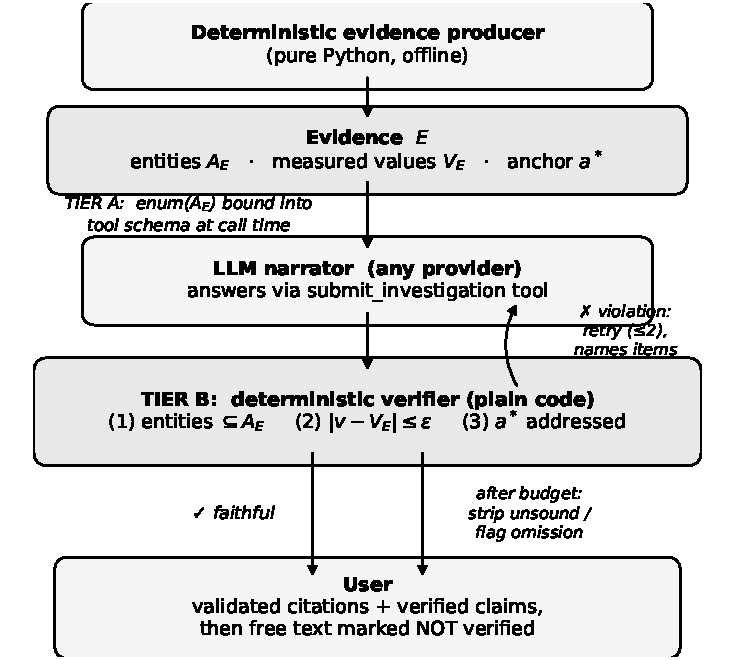
\includegraphics[width=\textwidth]{contract_flow.pdf}
\caption{The evidence-bound contract. The deterministic evidence producer
emits $E$; Tier~A binds the tool schema's enums to $E$ at call time; Tier~B
re-checks the returned answer in plain code on three channels, retries with
the offending items named, and after the budget strips unsound content and
flags a persistent omission. The bottom box states the scope honestly: the
validated channels carry the guarantee, and the free-text field reaches the
user too, marked as unverified.}
\label{fig:contract}
\end{figure}

Figure~\ref{fig:contract} draws the system the way the contract sees it. A
dashed trust boundary splits it in two. On one side is everything
deterministic: the pure-Python evidence producer, the dictionary $E$, the
Tier~B verifier, and the user-facing output, all plain code. On the other is
the \emph{LLM narrator}, which we treat as untrusted regardless of who serves
it. Every arrow crossing the boundary is contract traffic. Outbound, Tier~A
binds the tool-schema enums to $E$ at call time. Inbound, the narrator's
\texttt{submit\_investigation} payload enters only through Tier~B
verification, and on a violation the corrective retry crosses back with the
offending items named.

Inside mlcompass the boundary sits within a larger system: eleven pipeline
tools behind a CLI, a tool-integration server~\cite{mcp}, an autonomous agent,
and editor slash commands, all over a persistent project-context folder. Every
one of those surfaces routes through the same deterministic backend. Because
the evidence layer is deterministic and offline, every command works with the
narrator absent; the narrator only adds explanation, and the contract is what
makes that explanation safe to act on.

\paragraph{Where the guarantee does not reach, and why we say so here.} The
contract governs the narrator \emph{mlcompass itself invokes}. On the
tool-server surface there is no such narrator by design: the tools return the
evidence dictionary and the \emph{calling} model --- the one in the user
editor --- is the interpreter. That model is a narrator over the same evidence
and it is entirely ungoverned. So the honest statement is not that the guarded
path is the only path from evidence to user; it is that \textbf{mlcompass
guarantees the faithfulness of its own narration and cannot guarantee anyone
else}. Exporting an enforceable contract across a tool-server boundary --- so
that a client model consuming the evidence is held to the same check --- is
open, and Section~\ref{sec:conclusion} names it as future work.

\subsection{The three layers}

\paragraph{Layer 1: deterministic evidence producer.} A pure-Python module
reads the predictions table and assembles $E$ as described in
Section~\ref{sec:theory}.

\paragraph{Layer 2: strict-prompted narrator.} The narrator receives $E$ with
a system prompt stating the rules in words: cite only items that appear in
$E$; report every correlation as a structured claim copied exactly from $E$;
address the top-ranked candidate before committing to a verdict; abstain
(\texttt{cannot\_determine}) rather than guess. Section~\ref{sec:rq4}
measures what this layer is worth on its own.

\paragraph{Layer 3: the evidence-bound runtime schema.} Answers arrive through
a \texttt{submit\_investigation} tool.

\emph{Tier~A} restricts the tool's \texttt{columns\_referenced} items and
\texttt{claims[].column} field by JSON-schema \texttt{enum}s built at call
time from $E$.

\emph{Tier~B} re-checks the returned tool input in plain code, trusting no
one:
\begin{enumerate}
\item \textbf{Entity soundness} --- every column cited or claimed must be in
the evidence set.
\item \textbf{Value soundness} --- each claim \{column, statistic, value\}
must match the measured value within $0.005$, so two-decimal rounding passes
and a misquote fails.
\item \textbf{Completeness} --- a verdict other than
\texttt{cannot\_determine} must address the top-ranked candidate; an explicit
abstention is not an omission.
\end{enumerate}
A failed check earns the narrator a corrective retry naming the offending
items (budget~2). Whatever is still unsound afterwards is \emph{stripped}, a
persistent omission is \emph{flagged}, and completeness is re-checked after
stripping, because deleting an unsound claim can orphan the anchor.

\subsection{The invariant, and its scope}

The invariant is easy to state, and its scope has to be stated with it:
\emph{within the validated citation and claim channels}, any response the
contract returns cites only entities present in the deterministic evidence and
quotes only values equal to it, by construction, whoever the provider is.

The free-text fields carry no such guarantee. The renderer prints them, marked
as unverified, beneath the validated content, and the product also ships a
second, entirely ungoverned prose interpreter over the same evidence, labelled
the same way. We state this in the artifact description rather than only in
the limitations, because a guarantee whose scope is left to the reader is a
guarantee that will be over-read. Membership, comparison, anchor: the checks
are almost embarrassingly small, and that smallness is what decidability buys.

\section{Study Design}\label{sec:design}

\subsection{Empirical methodology, named}

Following the ACM SIGSOFT Empirical Standard for engineering research, we
state the method explicitly rather than leaving it to be inferred. RQ1--RQ4
are answered by a \textbf{controlled experiment} over a fixed evidence
dictionary, in which the only manipulated variable is the enforcement
mechanism (RQ1--RQ3) or the wording of an instruction (RQ4). RQ5 is answered
by a \textbf{benchmark} over pinned public datasets with a pre-registered
protocol, a frozen analysis plan, and an amendment log.

\subsection{Subject system and tasks}

The subject is the shipped leakage-investigation path of mlcompass. The
\emph{synthetic} task is a $1{,}000 \times 12$ regression frame carrying a
monotone transformed leak
($\texttt{log\_target\_v2} = \log(y) + \mathcal{N}(0, 0.01^2)$) and a
high-correlation distractor; ten evidence columns, anchor
\texttt{log\_target\_v2}. In every arm the \emph{shipped}
\texttt{detect\_leakage} produces $E$, so the narrator sees exactly the
evidence shape the product produces in the field.

For RQ5 the subjects are three pinned OpenML datasets --- 1464
(blood-transfusion, 748~rows), 1480 (ILPD, 583~rows) and 44031
(california, 20{,}640~rows) --- chosen for task-type spread and issue
diversity. Each is fetched to a checksummed local copy with its OpenML version
and file id recorded, and re-hashed before every run; a changed input is an
error rather than a surprise.

\subsection{Arms}

\paragraph{Contract and baseline arms (RQ1--RQ3), $N=200$ each.}
\begin{description}
\item[\texttt{A-L1}] The floor: bare prompt requesting the structured fields,
stating no faithfulness rule, open enum-free schema, no verification.
\item[\texttt{A-CONTRACT}] The shipped enforcement stack (Tier~A + Tier~B)
with the faithfulness \emph{prompt removed}, so the contract is compared to
bare-prompt baselines without confounding prompt with mechanism.
\item[\texttt{A-STRESS}] The shipped contract with the bare prompt \emph{and}
the Tier~A enums removed, so the narrator fabricates at its natural rate and
every Tier~B catch becomes observable.
\item[\texttt{A-GR-STOCK}] \textbf{Guardrails~AI} with structural validation
and reask only: what a validate-and-reask toolkit gives out of the box.
\item[\texttt{A-GR-OURS}] \textbf{Guardrails~AI running custom validators that
encode the Tier~B checks.} Our validator, their loop; the comparison is loops.
\item[\texttt{A-STRICT-STATIC}] The provider's strict structured-output mode
over a static schema carrying types and required fields and \emph{no} column
enum.
\item[\texttt{A-STATIC-ENUM-STALE}] The same strict mode with a column enum
declared once at author time instead of generated at call time.
\end{description}
Reask budget is 2 in every arm that has one, matching the contract's retry
budget, so no arm is given more attempts than another.

\paragraph{Paraphrase sweep (RQ4), $N=100$ per variant.} The bare instruction
rewritten six ways --- \emph{terse}, \emph{baseline}, \emph{cautious},
\emph{expert}, \emph{helpful}, \emph{mechanical} --- none containing a
faithfulness rule, over the same evidence and tool schema. All six were
written before any measurement and none was discarded afterwards. Only the
wording moves.

\paragraph{Downstream benchmark (RQ5), $3\times4\times3$ per arm.} Four arms,
each asked to write a training script for a pinned dataset:
\begin{description}
\item[\texttt{control}] The task, the CSV path, the target, the column
listing, and the list of installed packages.
\item[\texttt{control+revise}] The control prompt, then a second turn saying
only \emph{review the script you just wrote and fix any problems you find in
it}. No findings, no checklist, no concern named.
\item[\texttt{advise}] The control prompt plus an appended block carrying the
verbatim stdout of \texttt{mlcompass advise} on the same training file.
\item[\texttt{advise+audit}] The \texttt{advise} turn, then one revision round
carrying the verbatim stdout of \texttt{mlcompass audit} on \emph{that arm's
own} first-turn script.
\end{description}
The arm list is ordered so that each neighbouring pair isolates one thing:
\texttt{control}$\rightarrow$\texttt{control+revise} isolates the extra
attempt; \texttt{control}$\rightarrow$\texttt{advise} isolates the advice
block; \texttt{control+revise}$\rightarrow$\texttt{advise+audit} isolates what
the tool adds on top of an extra attempt.

\subsection{Measures}

\paragraph{Faithfulness channels (RQ1--RQ4).} Scored on every response that
reaches the user. \textbf{Entity fabrication}: at least one column, cited or
claimed, outside $E$. \textbf{Value fabrication}: at least one claim whose
column is in $E$ but whose value is off by more than $0.005$.
\textbf{Critical omission}: a committed verdict that never references the
anchor. We report Wilson 95\,\% intervals and raw $k/N$ throughout.

Section~\ref{sec:rq1} introduces a decomposition of the entity channel that we
did not have when the study began, and which changed what we believe the
channel measures:
\begin{description}
\item[invented] a name appearing \emph{nowhere} in $E$ --- the phantom entity
as the literature defines it;
\item[misfiled] a name that \emph{is} in $E$ but is not a column, written into
a field that holds only columns.
\end{description}
Both are contract violations and Tier~B rejects both identically; only the
first is a hallucination. The blended \textbf{entity} flag retains its original
meaning --- their disjunction --- so no comparison in this paper moves because
of the decomposition.

\paragraph{Downstream measures (RQ5).} A deterministic six-item checklist over
the emitted script --- \texttt{no\_seed}, \texttt{leak\_fit\_before\_split},
\texttt{leak\_duplicate\_rows}, \texttt{wrong\_metric\_for\_imbalance},
\texttt{no\_validation}, \texttt{target\_in\_features} --- plus whether the
script runs, and a held-out score obtained by the harness loading the model
the script saved and predicting on data the script never saw.

\subsection{Controls that the design turns on}

\paragraph{Holdout splitting on duplicate groups.} The pinned datasets contain
duplicate rows (125 retained inside train on OpenML~1464). A plain split put
71 of 187 holdout rows verbatim into train, so a script that correctly
de-duplicated scored \emph{below} one that did not. We split on groups of
identical rows: no holdout row appears verbatim in train, while duplicates
remain inside the training file, so the score is honest and the defect stays
reachable. This is recorded as amendment~A4 and is the single change that most
affected the benchmark's validity.

\paragraph{Stating the execution environment.} Every arm's prompt carries the
same generated list of importable packages. Without it, \texttt{runs\_at\_all}
partly measured package availability, and the confound had a direction:
advise output recommends handling class imbalance, which points at exactly the
resampling libraries most likely to be absent, so silence would have penalised
the treatment arm for taking the intervention's advice (amendment~A5).

\paragraph{Transport failures are not data.} A failed API call is excluded
from $N$ and reported per cell, rather than being counted as a clean
non-fabricating response. Section~\ref{sec:instruments} describes the incident
that makes this rule load-bearing.

\subsection{Pre-registration and amendments}

The downstream protocol was frozen before execution, including the arms, the
datasets, the models, the repetition count, the seeds, and --- in
Section~6 of the protocol --- the outcome we would regard as publishable if
the metric did not move. Every deviation is recorded as a numbered amendment
with its reason; eleven amendments (A1--A11) are in the replication package,
and the ones that changed a conclusion are discussed in
Section~\ref{sec:instruments} rather than buried in an appendix.

\subsection{Models and generation settings}

RQ1--RQ4 run on DeepSeek \texttt{deepseek-chat} over an OpenAI-compatible
endpoint with JSON-schema tool use. RQ5 runs a four-model panel:
\texttt{deepseek-flash}, \texttt{ministral-8b-latest},
\texttt{qwen2.5:7b} served locally by Ollama, and
\texttt{gpt-5.4-mini}. Temperature is fixed at $1.0$ on every arm and every
provider, sent explicitly in the request body rather than left to a provider
default, and recorded in every run record. Results are reported per model and
never pooled.

\section{RQ1: How Does an Unconstrained Narrator Actually Fail?}\label{sec:rq1}

\subsection{The blended rate, and why it is not the answer}

On the bare arm the narrator produced an out-of-evidence entity in
\textbf{42.0\,\%} of 200 responses (84/200, Wilson 95\,\% CI
$[35.4, 48.9]$). Read as published, that is a fabrication rate, and it is the
kind of number this literature reports.

It is not a fabrication rate. Decomposing every flagged response across all
seven arms of the battery --- 1{,}400 live responses --- gives
Table~\ref{tab:decomp}.

\begin{table}[t]
\caption{Decomposition of every flagged entity in the seven-arm battery
($N=200$ per arm, 1{,}400 responses). \emph{Invented} = the name appears
nowhere in $E$. \emph{Misfiled} = the name is in $E$ but is not a column.}
\label{tab:decomp}
\centering
\begin{tabular}{@{}lrrrl@{}}
\toprule
Arm & flagged & misfiled & \textbf{invented} & what was cited \\
\midrule
\texttt{A-L1}             & 84 & 84 & \textbf{0} & \texttt{r2}$\times$87, \texttt{perfect\_match\_rate}$\times$1 \\
\texttt{A-GR-STOCK}       & 70 & 70 & \textbf{0} & \texttt{r2}$\times$70 \\
\texttt{A-STRICT-STATIC}  &  8 &  8 & \textbf{0} & \texttt{r2}$\times$8 \\
every other arm           &  0 &  0 & \textbf{0} & --- \\
\midrule
total                     & 162 & 162 & \textbf{0} & \\
\bottomrule
\end{tabular}
\end{table}

\textbf{Across 1{,}400 live responses on this task the narrator invented
nothing.} Every flagged entity is \texttt{r2} --- the name of the suspicious
metric, which $E$ carries as \texttt{suspicious\_metric.name} and which the
model wrote into \texttt{columns\_referenced}.

\subsection{What this changes, and what it does not}

It changes what the number may be called. The failure mode this literature
names, and which we had set out to measure, is \emph{phantom-entity
fabrication}: ``a column the data does not contain''. On this evidence that is
not what the 42.0\,\% counts. A reviewer with these logs
would say the rate measures a category error, the model naming the metric it
was handed, and on this battery they would be right.

It does not change three things.

First, \textbf{it remains a contract violation.}
\texttt{columns\_referenced} means columns of the data. A consumer acting on
\texttt{r2} --- dropping it, correlating it, listing it as a leak candidate ---
acts on something that does not exist as a column. Rejecting it is correct
behaviour, not over-eager behaviour.

Second, \textbf{it does not affect any arm comparison.} Every arm faced the
same failure; Section~\ref{sec:rq3} separates them from 42.0\,\% to 0/200
regardless of the provenance of the name.

Third, and most importantly, \textbf{invention is not absent in general} ---
only on this task under these prompts. Section~\ref{sec:rq4} finds it, at a
much lower rate and, unexpectedly, moving in a different direction from the
blended rate.

\subsection{The zeros are not cheap}

Value fabrication and critical omission were 0/200 in all seven arms. A
narrator that escaped into abstention would score zero on every channel for
free, so we measured whether it did (Table~\ref{tab:abstain}).

\begin{table}[t]
\caption{The silent channels are silent because the narrator committed, not
because it declined. $N=200$ per arm.}
\label{tab:abstain}
\centering
\begin{tabular}{@{}lrr@{}}
\toprule
 & \texttt{A-L1} & \texttt{A-CONTRACT} \\
\midrule
Abstained (\texttt{cannot\_determine} or equivalent) & 2/200 & 0/200 \\
Claims per response, median                          & 10    & 10 \\
Never mentioned the anchor                           & 0/200 & 0/200 \\
\bottomrule
\end{tabular}
\end{table}

The narrator commits, and commits to ten structured claims per response. A
zero here is therefore a measurement and not an artefact of a narrator that
declined to speak.

\section{RQ2 and RQ3: Prevention, and Whether It Beats the Alternatives}\label{sec:rq3}

\subsection{Results}

Table~\ref{tab:arms} is the head-to-head. All seven arms share the task, the
evidence, the model, the reask budget and the scoring; they differ only in the
enforcement mechanism.

\begin{table}[t]
\caption{User-facing entity-fabrication rate, seven arms, $N=200$ each,
DeepSeek \texttt{deepseek-chat}, 2026-09-15. Wilson 95\,\% intervals.}
\label{tab:arms}
\centering
\begin{tabular}{@{}llrcr@{}}
\toprule
Arm & Mechanism & Rate & 95\,\% CI & $k/N$ \\
\midrule
\texttt{A-L1}            & no enforcement                         & 42.0\,\% & [35.4, 48.9] & 84/200 \\
\texttt{A-GR-STOCK}      & Guardrails AI, stock validators        & 35.0\,\% & [28.7, 41.8] & 70/200 \\
\texttt{A-STRICT-STATIC} & provider strict mode, no enum          &  4.0\,\% & [2.0, 7.7]   &  8/200 \\
\midrule
\texttt{A-GR-OURS}       & \textbf{Guardrails' loop, our Tier B}   & \textbf{0.0\,\%} & [0.0, 1.9] & 0/200 \\
\texttt{A-CONTRACT}      & Tier A + Tier B                        & \textbf{0.0\,\%} & [0.0, 1.9] & 0/200 \\
\texttt{A-STRESS}        & Tier B alone, no enum                  & \textbf{0.0\,\%} & [0.0, 1.9] & 0/200 \\
\texttt{A-STATIC-ENUM-STALE} & strict mode, author-time enum      & 0.0\,\%$^{\dagger}$ & [0.0, 1.9] & 0/200 \\
\bottomrule
\end{tabular}
\\[2pt]
\footnotesize $^{\dagger}$Degenerate on this task --- see
Section~\ref{sec:rq3-degenerate}. The row carries no comparison.
\end{table}

\subsection{It is the validator, not the loop}

The two rows to read together are \texttt{A-GR-STOCK} and \texttt{A-GR-OURS}.
\textbf{The same toolkit, the same reask loop, the same budget of two, the same
model, the same prompt: 35.0\,\% against 0/200.} The only thing that changed is
what the validator checks.

Guardrails' structural validators confirm the answer has the right shape. They
have no way to know which column names the evidence contained, because nothing
told them --- and nothing could, without the call-time binding that is the
contract's first tier. This is the paper's central empirical claim, and it is
now measured against the nearest real alternative instead of asserted:
\textbf{the outer loop is general-purpose infrastructure and was never the
contribution; the validator inside it is.}

\texttt{A-STRESS} reaching 0/200 with the enum removed says the same thing
from the other side. Post-generation verification alone suffices, which is what
makes the guarantee independent of the provider. Tier~B fired on 12 of 200
responses in that arm and passed none of them through.

\texttt{A-GR-OURS} is the instructive middle: Tier~B's checks caught 86
violations across 84 responses inside Guardrails' loop, and the user-facing
rate was still 0/200. The loop is a perfectly adequate delivery vehicle for a
decidable check. It just does not contain one.

\subsection{Provider strict mode is close, and uncertifiable}\label{sec:rq3-degenerate}

\texttt{A-STRICT-STATIC} reaches 4.0\,\%: a static schema with types and
required fields and no column enum leaves the column domain unconstrained, so
any out-of-domain name decodes successfully. That it lands at 4\,\% rather than
42\,\% is evidence that a schema \emph{steers} a model strongly even where it
does not constrain it --- the same effect we report for Tier~A in
Section~\ref{sec:rq4}. Steering is not enforcement, and cannot be certified:
it can regress as silently as a prompt.

\texttt{A-STATIC-ENUM-STALE} must not be read as a result. On this task the
author-time column list covers 10 of 10 evidence columns, so the arm is
byte-identical to a live enum \emph{by construction}. The harness detects and
reports this degeneracy at plan time. The arm is informative only on a task the
frozen list predates, and no such task is in this battery; the row is printed
for completeness and carries no comparison. We report this rather than quietly
omitting the row, because a 0/200 cell that looks like a win and is an identity
is exactly the kind of number a reader should be warned about.

\section{RQ4: Can a Prompt-Level Defence Be Certified?}\label{sec:rq4}

\subsection{Results}

Table~\ref{tab:sweep} reports the six-variant sweep: one instruction, six
rule-free rewordings, $N=100$ each, zero transport errors, same evidence and
same tool schema. Only the wording moves.

\begin{table}[t]
\caption{Paraphrase sweep, $N=100$ per variant, 600 live responses. The
blended rate and the invention count are reported separately because they do
not move together.}
\label{tab:sweep}
\centering
\begin{tabular}{@{}lrcrrl@{}}
\toprule
Variant & Entity-fab & 95\,\% CI & $k/N$ & \textbf{invented} & misfiled \\
\midrule
terse      &  9.0\,\% & [4.8, 16.2]  &  9/100 & \textbf{7} &  4 \\
baseline   & 36.0\,\% & [27.3, 45.8] & 36/100 & \textbf{0} & 36 \\
expert     & 57.0\,\% & [47.2, 66.3] & 57/100 & \textbf{7} & 51 \\
cautious   & 68.0\,\% & [58.3, 76.3] & 68/100 & \textbf{2} & 68 \\
helpful    & 71.0\,\% & [61.5, 79.0] & 71/100 & \textbf{5} & 71 \\
mechanical & 72.0\,\% & [62.5, 79.9] & 72/100 & \textbf{1} & 71 \\
\bottomrule
\end{tabular}
\end{table}

Three readings.

\paragraph{Wording moves the blended rate roughly eightfold.} From 9.0\,\% to
72.0\,\%, across six variants written before any measurement with none
discarded afterwards, on identical evidence with no faithfulness rule in any of
them. A terse instruction almost never trips the check. A mechanical
field-listing instruction almost always does. No obvious feature of the wording
predicts where a variant will fall.

\paragraph{Invention exists here, at an order of magnitude below the
headline.} Five of six variants produced names absent from $E$ entirely --- the
frame's ten columns are \texttt{log\_target\_v2}, \texttt{near\_target\_proxy}
and \texttt{feature\_4}\ldots\texttt{feature\_12}, and there is no column
called \texttt{target}, so a response citing
\texttt{[log\_target\_v2, near\_target\_proxy, target]} invented the third.
Phantom-entity fabrication is therefore real and not an artefact of the
scorer. It occurs at 0--7 per 100, not at the 36--72\,\% the blended rate
reports.

\paragraph{The two channels move independently, and at the extremes they
run opposite.} This was not expected and is the sharper finding:

\begin{center}
\footnotesize
\begin{tabular}{@{}lrr@{}}
\toprule
variant & blended & invented \\
\midrule
terse      &  9\,\% & 7 \quad $\leftarrow$ lowest blended, highest invented \\
baseline   & 36\,\% & 0 \quad $\leftarrow$ zero inventions at 36\,\% \\
expert     & 57\,\% & 7 \\
cautious   & 68\,\% & 2 \\
helpful    & 71\,\% & 5 \\
mechanical & 72\,\% & 1 \quad $\leftarrow$ highest blended, near-zero invented \\
\bottomrule
\end{tabular}
\end{center}

The mechanism is legible. A field-listing instruction drives the model to
enumerate evidence fields, which produces misfiling, not invention. A terse
instruction says little and the model fills the gap from somewhere other than
$E$.

\subsection{Interpretation}

The manuscript's thesis is that a prompt-level defence cannot be certified from
observed compliance. The decomposition makes that claim harder, not softer:
\textbf{you cannot even certify one failure mode from another within the same
prompt.} The wording that looks safest on the headline metric is the one
inventing most. An engineer choosing a prompt by measuring its fabrication rate
would choose \emph{terse} and would be choosing the variant that most often
invents a column that does not exist.

Abstention was checked here too, for the same reason as in
Section~\ref{sec:rq1}: 1, 2, 0, 1, 0 and 8 per 100 across the six variants. The
low cells are low because the model cited cleanly, not because it declined to
answer.

Two further diagnostic arms pull the tiers apart. Placing the evidence-bound
enum in the schema over a bare prompt with no verification --- Tier~A alone ---
drove the rate to 0/200, and running the full contract under the sweep's worst
paraphrase produced zero first-attempt violations and therefore zero catches.
Neither observation is a guarantee: steering can regress as silently as
prompting. Together with \texttt{A-STRESS} they give a consistent picture ---
each tier is independently effective in practice, and Tier~B is the only layer
whose protection is certifiable.

\section{RQ5: Does the Tool Change What the Model Produces?}\label{sec:rq5}

\subsection{Results}

Table~\ref{tab:ab} reports the downstream benchmark: 144 runs, four models,
three datasets, three repetitions, four arms, all on one frozen split per
dataset.

\begin{table}[t]
\caption{Flagged defects, summed over the nine runs of each (model, arm) cell.
Scoring version \texttt{rescored-v2}; see Section~\ref{sec:instruments} for the
two scorer corrections applied to the same preserved scripts.}
\label{tab:ab}
\centering
\begin{tabular}{@{}lrrrr@{}}
\toprule
Model & \texttt{control} & \texttt{control+revise} & \texttt{advise} & \texttt{advise+audit} \\
\midrule
deepseek-flash        & 13 & 11 & 13 & \textbf{4} \\
ministral-8b          &  8 &  6 &  3 & \textbf{0} \\
qwen2.5-7b (local)    &  6 &  9 &  4 & \textbf{1} \\
gpt-5.4-mini          &  6 &  9 &  6 & \textbf{3} \\
\midrule
\textbf{total}        & \textbf{33} & \textbf{35} & \textbf{26} & \textbf{8} \\
\bottomrule
\end{tabular}
\end{table}

\subsection{The extra attempt is worth nothing; the findings are worth
$33 \rightarrow 8$}

The obvious objection to a treatment arm that revises is that it differs from
the control in \emph{two} ways at once: it is told what is wrong, and it gets a
second attempt. Our first version of this benchmark could not separate them,
and the objection was raised in internal review before it could be raised
externally. The \texttt{control+revise} arm exists to answer it.

A second attempt on its own does nothing: $33 \rightarrow 35$, two models down
and two up, noise around no effect. The within-arm view is sharper. Across the
35 runs that produced a defect count on both sides of the revision turn:

\begin{center}
\begin{tabular}{@{}lr@{}}
\toprule
unchanged & 33 \\
worse     & 2 \\
better    & \textbf{0} \\
\bottomrule
\end{tabular}
\end{center}

\textbf{Self-revision without the tool's findings did not repair a single
defect in 35 runs.} The model was handed its own script and asked to find
problems in it, and found none it could act on --- while the same models, shown
\texttt{mlcompass audit} output on the same kind of script, fix them. The fall
from 33 to 8 is attributable to the findings and not to the turn they arrive
with.

\subsection{The held-out score shows no consistent improvement}

Across the nine (model, dataset) cells with both ends scored, the held-out
score moved better in three, worse in three, and within $\pm0.01$ in three. No
direction. The spread inside an arm frequently exceeds the gap between arms:
one arm spans $0.2122$ across three repetitions while its median sits $0.0002$
above control.

We state the conclusion at the strength the data supports.
\textbf{No consistent improvement in held-out score could be shown.} That is not the same as showing there is no
effect, and with only 70 of 108 runs carrying a score --- 21 scripts failed to
run, 17 saved artefacts the scorer could not load, and 8 of 36 cells carry no
score at all --- this design cannot establish a null. Section~6 of the frozen
protocol named ``the process improves, the metric does not'' as a probable and
publishable outcome \emph{before any data existed}, and nothing here refuted
it; but a pre-registered prediction that survives is not a measured null, and
we do not report it as one.

\section{Three Defects in Our Own Instruments}\label{sec:instruments}

Every number in this paper is produced by an instrument we wrote. We found
three defects in those instruments while running the study, two of them after
results had already been drawn from them, and all three are reported here
rather than in an appendix because each changed something a reader would
otherwise take at face value. The replication package preserves the original
scoring beside every correction, so a reader can recompute either.

\subsection{Defect 1: the checklist penalised correct code, in a biased
direction}

The downstream checklist scores the \emph{absence} of every enumerated way of
excluding the target column from the feature matrix. The enumeration did not
include a list comprehension:

\begin{quote}\ttfamily\small
target\_col = "Class"\\
feature\_cols = [c for c in df.columns if c != target\_col]\\
X = df[feature\_cols]
\end{quote}

This script excludes the target and was scored \texttt{target\_in\_features:
yes}. Fifteen of 108 runs carried the false positive. Two further forms were
found later by the same route: a feature list assembled from named constants
(\texttt{FEATURE\_COLS = NUMERIC\_COLS + CATEGORICAL\_COLS}) and a seed hoisted
to a module constant (\texttt{RANDOM\_STATE = 42}, passed in three places,
scored \texttt{no\_seed}).

The shape of the rule is the defect, not any single missing pattern. An
absence-scored checklist has an open-ended form list, so every form nobody
enumerated becomes a false positive on correct code. \textbf{And the bias has a
direction.} Tidier code hoists lists and seeds to constants; a revised script
is a tidier script; so the checker systematically penalised the coding style
that the treatment arms produce.

Corrected against the same bytes --- no model call, no re-execution, dataset
facts read back from each run's record --- across two rescoring passes:

\begin{center}
\begin{tabular}{@{}lrrr@{}}
\toprule
scoring & \texttt{control} & \texttt{advise} & \texttt{advise+audit} \\
\midrule
original            & 40 & 31 & 15 \\
after correction 1  & 35 & 27 &  9 \\
after correction 2  & \textbf{33} & \textbf{26} & \textbf{8} \\
\bottomrule
\end{tabular}
\end{center}

The direction survives all three scorings. It has also moved toward our
hypothesis three times running, and we say so plainly rather than burying it:
false positives concentrate in careful code and the treatment arms produce more
careful code, which is a checkable mechanism rather than an excuse. A reader
should verify it rather than accept it. The next correction that moves these
numbers the other way will be the one indicating the scorer is finally
unbiased.

\subsection{Defect 2: a provider change silently emptied every cell}

The contract harness pins a default model per provider. A pin was updated on a
deprecation notice and never exercised. Every current model at that provider is
a reasoning-mode model, and reasoning mode refuses the forced
\texttt{tool\_choice} the contract requires:

\begin{quote}\ttfamily\small
400 --- Thinking mode does not support this tool\_choice
\end{quote}

so every call failed at transport and every cell reported $0.0\,\%$ with $k/N$
of $0/0$.

The exclusion rule of Section~\ref{sec:design} is what made this visible rather
than catastrophic: transport failures were excluded from $N$ rather than
counted as clean non-fabricating responses, so the tables showed a hole instead
of a false success. That rule had been added after an earlier review found a
failed run scored as a success, and it earned its keep here.

One detail is worth recording for others building such harnesses: the model
that \emph{does} accept the call is absent from the provider's
\texttt{models.list()} endpoint while still being served. Probing the listing
would have confirmed the wrong conclusion. The only reliable check is to send
the call shape the system actually uses.

\subsection{Defect 3: the pre-registration was not enforced, and the tooling
caused the violation}

The downstream protocol rests on freezing a plan before execution. For one run
that discipline was decorative: the runner checked only that a plan file
\emph{existed}, then ran whatever the command line said. A plan froze twelve
cells of one arm at three repetitions --- 36 runs --- and the execution
performed 48 runs across all four arms at one repetition, wrote them under the
plan's own identifier, and exited successfully.

The cause was not carelessness at the keyboard. On freezing a plan the tool
printed:

\begin{quote}\ttfamily\small
Run it with:\\
\ \ python run\_ab.py --experiment-id <id> --panel-id <p> ...
\end{quote}

carrying neither the arm selection nor the repetition count. \textbf{Following
the tool's own instruction guaranteed the mismatch.} A pre-registration whose
tooling hands the author the command that breaks it is a paragraph, not a
method.

The plan's cell table is now parsed back into the arms, datasets, models,
repetitions and seeds it commits to, and the runner aborts --- naming every
divergence, before anything executes or is written --- if the run about to
start is not the run the plan froze. The check runs before the dry-run listing
returns, because a violation discoverable only by spending money is not a
check. The 48 rows were relabelled rather than deleted, with a note stating
what happened, and the arm was rerun against the enforced plan.

\subsection{Defect 4: a point estimate is a property of a date}

A pilot battery run three months earlier, on the same task and the same
provider family with the same scorer, measured the bare-arm entity rate at
11.5\,\%, CI $[7.8, 16.7]$. The battery reported here measures 42.0\,\%,
CI $[35.4, 48.9]$ --- far outside that interval. The pilot measured the
paraphrase sweep span as 1\,\% to 100\,\%; this study measures 9\,\% to
72\,\%.

We cannot reconcile them, and we are not going to pretend otherwise. Both pilot
figures were obtained against a \emph{rolling model alias}, and their
per-response records were not retained, so there is nothing left to recompute.
What we can say is what the discrepancy implies for anyone reading rates of
this kind, our own included.

First, \textbf{a fabrication rate is a property of a model version at a date,
not of a model.} Reporting a point estimate and a confidence interval against a
rolling alias produces a number that cannot be reproduced even by its own
authors, and the interval invites a precision the design does not support. We
treat this as a threat to validity in its own right
(Section~\ref{sec:threats}), and it is the reason every cell in this paper
pins a model string, a date, and a harness commit, and retains one record per
response.

Second, \textbf{the qualitative claims are the ones that survived the
instability.} Rewording still moves the rate by roughly an order of magnitude;
the contract still returns 0/200; the stock-validator baseline still leaves a
third of responses unfaithful. Results built on qualitative invariants outlived
a fourfold change in the underlying rate, and results built on point estimates
did not. We recommend the former, and have written this paper accordingly.

All 2{,}000 per-response records behind the present study are in the
replication package.

\section{Discussion}\label{sec:discussion}

\subsection{Prompts are advisory; schemas with verification are enforcement}

The sweep turns a slogan into a number. One model, one evidence dictionary, and
a rate anywhere between 9\,\% and 72\,\% depending on harmless wording choices.
The strict prompt's zeros are real, and they still leave a 1.9\,\% Wilson upper
bound with nothing structural holding them in place across the next model
update or the next paraphrase. The contract supplies what no prompt can: a
worst-case guarantee at any propensity, under any wording, on the channels it
validates.

Section~\ref{sec:rq3} is what upgrades this from a slogan to a comparison. Had
\texttt{A-GR-OURS} landed at 20\,\% we would have learned that the loop matters
and our validator is one of several adequate ones. It landed at 0/200 with the
same loop that leaves 35\,\% under stock validators, which locates the
contribution precisely: not a better reask loop, but a decidable check that a
general-purpose loop cannot express because nothing tells it what the evidence
contained.

\subsection{Detection enables correction}

The stress arm carries a second lesson. The verifier does more than block: it
names what went wrong, and machine-generated violation reports are a strong
mitigation in their own right. Contrast the \emph{cautious} paraphrase --- which
amounts to telling the model to be careful --- at 68\,\%. Vague guidance is
weak; precise deterministic feedback is strong. The division of labour follows:
let the verifier, not the prompt author, do the correcting.

RQ5 is the same lesson at a larger scale and with the confound removed. Asking
a model to review its own script repaired zero defects in 35 runs. Handing it a
deterministic tool's findings about that script moved four model lanes from 33
flagged defects to 8. What the tool contributes is not encouragement to be
careful; it is a specific, checkable statement of what is wrong.

\subsection{Negative results are boundaries, not failures}

Nothing fired on the value and omission channels anywhere in the battery, and
we did not read that as a victory. The honest explanation is that the numbers
sit verbatim in the context window, copying them is easy, and the anchor is the
most salient item in $E$. Longer contexts, derived statistics, or busier
evidence could activate either channel. The contract closes both pre-emptively
at the price of a set lookup and a float comparison
(Proposition~\ref{prop:linear}). Paying that price before a channel is observed
to fail, rather than after, is the right default for evidence-closed narrators.

The held-out score in RQ5 is the other negative result, and the more important
one for practitioners: \emph{the process improves and the metric does not
follow}. A tool that measurably reduces defects in generated training code did
not measurably improve the models those scripts produce. Both halves belong in
the report.

\subsection{Where the contract transposes}

Three invariants make it portable: a deterministic evidence producer, a finite
enumerable set of observed entities and values, and a runtime enum bound to
that set with independent verification. Any narration task with all three
supports the same guarantee. A clinical-decision narrator could be bound to the
patient's actually-measured abnormal results, with cited values verified against
the measurements; an expert-system narrator could be bound to the identifiers
of the rules that fired. We have not evaluated either domain, and they mark
where our claims stop.

One engineering note from shipping: when a capability is exposed through
several interfaces --- a CLI and a tool server here --- parity must be enforced
through shared code paths and tested as an invariant. We hit and fixed exactly
such a divergence.

\section{Threats to Validity}\label{sec:threats}

\subsection{Construct validity}

\paragraph{The entity channel measures two things.} This is the threat
Section~\ref{sec:rq1} exists to address. Until we decomposed it, a rate
reported as \emph{fabrication} was dominated by misfiling. We now report both
and keep the blended flag only for continuity with the arm comparisons. Any
reader comparing our rates to another paper's should check which of the two
that paper counts; we suspect the distinction is not made elsewhere.

\paragraph{The downstream checklist is an absence-scored proxy.} Six
deterministic rules are not ``code quality''. They are six things that are
cheap to check and expensive to get wrong, and Section~\ref{sec:instruments}
shows how the absence-scoring shape produces false positives with a direction.
Two independent raters blind to arm would be a stronger instrument; we did not
have them.

\paragraph{Free text is unmeasured.} The guarantee covers the validated
citation and claim channels. Enforcement pressure could push fabrication into
the unverified prose field, and we did not measure such displacement.
Miscalibrated confidence on correctly-cited, correctly-valued evidence is also
unscored.

\subsection{Internal validity}

\paragraph{Provider non-determinism.} Temperature is fixed at $1.0$ and sent
explicitly, but the endpoints are closed and may change beneath a stable model
name. Section~\ref{sec:instruments} documents two of our own figures that a
later run did not reproduce for what we believe is exactly this reason.

\paragraph{Repetitions share a split.} The three repetitions of each downstream
cell use one split per dataset, so they measure generation variability and not
split variability. A design varying both would be stronger and is future work.

\paragraph{The stress arm's propensity is not the bare arm's.} It reuses the
shipped contract's user message, which mentions a contract, so its first-attempt
propensity differs from \texttt{A-L1}'s. We report its catches as
demonstrations that the verifier fires, not as estimates of a bare rate.

\subsection{External validity}

\paragraph{One task family for the contract.} RQ1--RQ4 use one synthetic
leakage task with one leak pattern. Other evidence shapes and other leak
patterns are unmeasured.

\paragraph{Provider coverage is uneven.} RQ1--RQ4 are single-provider. RQ5 uses
four models across three providers plus a local model, which is where the
generalisation evidence in this paper lives. Rates should not be transferred
between providers; our own sweep shows they do not even transfer across
paraphrases of one prompt.

\paragraph{Datasets are small and tabular.} Three OpenML datasets, 583 to
20{,}640 rows. Nothing here speaks to deep-learning pipelines, to which the
audit rules largely do not apply.

\subsection{Conclusion validity}

\paragraph{Seventy of 108 runs carry a held-out score.} Eight of 36 cells carry
none. We therefore report ``no consistent improvement could be shown'' and
decline to report a null. No decision rule for ``beats'' was pre-registered,
and with medians separated by $0.0002$ that, rather than the amount of data, is
the binding constraint on any stronger claim.

\paragraph{Corrections have run one way.} Three scorer corrections have each
moved the downstream numbers toward our hypothesis. The mechanism is stated and
checkable in Section~\ref{sec:instruments}; we flag the pattern explicitly so a
reader can weigh it.

\section{Conclusion}\label{sec:conclusion}

Evidence-closed narration names the class of tasks whose citable entities and
verifiable quantities are finite and machine-enumerable at call time. For this
class, faithfulness checking is linear-time
(Proposition~\ref{prop:linear}); soundness can be enforced by safe deletion
while completeness can only be detected
(Proposition~\ref{prop:asym}, a transposition of a classical database-repair
result with a safety argument added); and fabrication on the verified channels
is therefore preventable rather than merely mitigable.

We measured a two-tier contract built on those facts, in the production path of
an open-source tool. Against the nearest real alternative, the finding is that
the outer loop was never the contribution: Guardrails~AI's own validators leave
35.0\,\% of responses unfaithful and the same loop running our deterministic
validators leaves 0/200. Against six rule-free rewordings of one instruction,
the failure rate moves from 9\,\% to 72\,\% --- and the invention rate moves
independently of it, so the wording that looks safest on the headline metric is
the one inventing most. Downstream, across four models and three datasets,
flagged defects fall from 33 to 8, and a fourth arm shows the fall is the
tool's findings and not the extra attempt they arrive with: self-revision
without findings repaired nothing in 35 runs.

We are explicit about what is claimed: not a new decoding algorithm, but a
decidable-class framing, a contract carrying one complexity observation and one
transposed repair asymmetry, and measurements of a shipped system against the
alternatives a practitioner would otherwise use. We are equally explicit about what
this study revised in our own understanding of the system it measures: the
failure mode is not the one we set out to find, a fabrication rate we had
measured once did not reproduce, and the downstream effect required a fourth
arm before it could be attributed to the tool at all.

The programme ahead is concrete: a public narrator-fabrication benchmark across
providers, tasks and leak patterns; verified claims over derived and relational
statistics; contract composition along multi-step agent chains, each step's
enum derived from the verified output of the step before, for which
assume-guarantee composition across agent boundaries~\cite{zheng2026continuity}
is the nearest existing machinery; a paired comparison against a
template-generated, LLM-free narration of the same evidence, which is the
experiment most likely to tell us what the language model is contributing that
a deterministic renderer would not; and an enforceable contract that survives
export across a tool-server boundary, so that a client model consuming a
tool own evidence is held to the same check as the tool internal narrator.

\backmatter

\section*{Statements and Declarations}

\paragraph{Funding.} No funding was received for conducting this study.

\paragraph{Competing interests.} The authors declare no competing interests.
mlcompass is released by the authors under the MIT licence and is not a
commercial product.

\paragraph{Author contributions.} H.S. designed and implemented the contract
and the measurement harnesses, and ran the batteries. Y.\"U. designed the
downstream benchmark protocol and performed the independent review that
identified the scorer false positives and the confound addressed in
Section~\ref{sec:rq5}. S.A. supervised the work. All authors read and approved
the final manuscript.

\paragraph{Data availability.} The replication package contains the source of
the artifact, every harness, every frozen protocol and amendment log, one
record per live response (2{,}000 records), every emitted script with its
verbatim model reply and execution output, and the scoring of every run
including the superseded scorings preserved beside their corrections. It will
be archived on Zenodo with a DOI on acceptance, under CC-BY~4.0 for data and
the MIT licence for code. The development repository is
\url{https://github.com/hakansabunis/mlcompass}.

\paragraph{Use of AI tools.} The authors used an LLM-based coding assistant
during implementation of the artifact and the harnesses, and during manuscript
preparation. All experimental design decisions, all interpretations of results,
and all claims in this paper are the authors'. Every number reported here was
produced by executing the committed harnesses over the committed evidence and
can be recomputed from the replication package; none was transcribed from a
model's summary.

\bibliography{references}

\end{document}
